%\documentclass{beamer} %voce pode usar este modelo tambem
\documentclass[t,handout,9pt]{beamer}
\usepackage{graphicx}
\usepackage{url}
\usepackage[british]{babel}
\batchmode
% \pgfpagesuselayout{4 on 1}[letterpaper,landscape,border shrink=5mm]
\usepackage{amsmath}
\usepackage{amssymb}
\usepackage{amsfonts}
\usepackage{enumerate}
\usepackage{epsfig}
\usepackage{bbm}
\usepackage{calc}
\usepackage{adjustbox}
\usepackage{color}
\usepackage{ifthen}
\usepackage{capt-of}
\usepackage{float}
\usepackage{booktabs}
\usepackage{dcolumn}
\usepackage{multicol}
\usepackage{hyperref}
\usepackage[flushleft]{threeparttable}
\usepackage{subcaption}
\usepackage{adjustbox}
\usepackage{ragged2e}
\usepackage{xcolor}
\usepackage{pgfpages}

\usepackage{pifont}
\newcommand{\cmark}{\ding{51}}%
\newcommand{\xmark}{\ding{55}}%

\usepackage{cmbright}

\renewcommand\ttdefault{cmvtt} % selects CM typewriter

\usepackage[utf8]{inputenc} % Required for inputting international characters
\usepackage[T1]{fontenc} 	% Output font encoding for international characters

%\DeclareFontShape{OT1}{cmss}{b}{n}{<->ssub * cmss/bx/n}{}

\usetheme[compress]{Berlin}
\definecolor{sapienza}{RGB}{0, 49, 83}
\usecolortheme[named=sapienza]{structure}

\usepackage[backend=bibtex,style=alphabetic,giveninits=true,url=false,eprint=false,doi=false]{biblatex}
\DeclareNameAlias{sortname}{last-first}
\renewcommand*{\nameyeardelim}{\addcomma\addspace}
\renewcommand*{\bibfont}{\footnotesize}
\addbibresource{example.bib}
\setbeamerfont{footnote}{size=\tiny}

\setbeamerfont{title}{size=\LARGE}

% reduce spaces between tables/figures and caption
\usepackage[font=small,skip=1pt]{caption}

%% pgf plots stuff
%\usepackage{pgfplots}
%\pgfplotsset{compat=newest}
%% the following commands are needed for some matlab2tikz features
%\usetikzlibrary{plotmarks}
%\usetikzlibrary{arrows.meta}
%\usepgfplotslibrary{patchplots}

% one navigation dot per slide trick
\AtBeginSection[]{\subsection{}}

% fix misbehave for allowframebreaks
\usepackage{etoolbox}
\makeatletter
\patchcmd{\slideentry}{\ifnum#2>0}{\ifnum2>0}{}% replace the subsection number test with a test that always returns true
% use frame numbers instead of subsection slide numbers so that frames broken over slides get separate circles
\patchcmd{\slideentry}{\c@subsectionslide}{\c@framenumber}{}{\@error{unable to patch}}
\patchcmd{\beamer@writeslidentry}{\c@subsectionslide}{\c@framenumber}{}{\@error{unable to patch}}

% date in footer trick
\makeatletter
  \setbeamertemplate{footline}{%
    \begin{beamercolorbox}[colsep=1.5pt]{upper separation line foot}
    \end{beamercolorbox}
    \begin{beamercolorbox}[ht=2.5ex,dp=1.125ex,%
      leftskip=.3cm,rightskip=.3cm plus1fil]{author in head/foot}%
      \leavevmode{\usebeamerfont{author in head/foot}\insertshortauthor}%
      \hfill%
      {\usebeamerfont{institute in head/foot}\usebeamercolor[fg]{institute in head/foot}\insertshortinstitute}%
    \end{beamercolorbox}%
    \begin{beamercolorbox}[ht=2.5ex,dp=1.125ex,%
      leftskip=.3cm,rightskip=.3cm plus1fil]{title in head/foot}%
      {\usebeamerfont{title in head/foot}\insertshorttitle\hfill\insertshortdate}%
    \end{beamercolorbox}%
    \begin{beamercolorbox}[colsep=1.5pt]{lower separation line foot}
    \end{beamercolorbox}
  }
\makeatletter

% remove dot for titlepage and Outline
\makeatletter
\let\old@beamer@writeslidentry\beamer@writeslidentry
\def\beamer@writeslidentry{%
  \expandafter\beamer@ifempty\expandafter{\beamer@framestartpage}{}% does not happen normally
  {%else
    \clearpage\beamer@notesactions%
  }
}
\makeatother

% let's number figure captions
\setbeamertemplate{caption}[numbered]

% trick for grouping equations
\newenvironment{rcases}
  {\left.\begin{aligned}}
  {\end{aligned}\right\rbrace}

%-------------------------Titulo/Autores/Orientador------------------------------------------------
\title[Introduction to Computer Programming]{Introduction to Computer Programming}
\date[A.Y. 2024-2025]{\\A.Y. 2024-2025}
\author[Alessio Martino]{Prof. Alessio Martino\\
\smallskip
{\small \href{mailto:amartino@luiss.it}{\texttt{amartino@luiss.it}}}\\
\smallskip
}
\institute[19/11/2024]{Department of Business and Management\\Viale Romania 32, 00197 Rome\\[\bigskipamount]

\includegraphics[scale=0.4]{Figures/cliente-luiss.png}%
}

%-------------------------Logo na parte de baixo do slide------------------------------------------
%\pgfdeclareimage[height=0.7cm]{senac-logo}{senac-logo.pdf}
%\logo{\pgfuseimage{senac-logo}\hspace*{0.5cm}}

%-------------------------Este código faz o menuzinho bacana na parte superior do slide------------
%\AtBeginSection[]
%{
%  \begin{frame}<beamer>
%    \frametitle{Outline}
%    \tableofcontents[currentsection]
%  \end{frame}
%}
%\beamerdefaultoverlayspecification{<+->}
% -----------------------------------------------------------------------------

\begin{document}
% -----------------------------------------------------------------------------

%---Gerador de Sumário---------------------------------------------------------

\frame[noframenumbering]{
	\titlepage
}

% begin personalization stuff
\setbeamertemplate{navigation symbols}{%
	\insertslidenavigationsymbol
	\insertframenavigationsymbol
	\insertsubsectionnavigationsymbol
	\insertsectionnavigationsymbol
	\insertdocnavigationsymbol
	\insertbackfindforwardnavigationsymbol
	\hspace{1em}%
	\usebeamerfont{footline}
	\insertframenumber/\inserttotalframenumber%
}
\setbeamertemplate{itemize items}[circle]
\setbeamertemplate{enumerate items}[circle]
\setbeamertemplate{bibliography item}{\insertbiblabel}
% end personalization stuff

\section[]{}
%\begin{frame}{Outline}
%	\tableofcontents
%\end{frame}
\begin{frame}{Outline}
\begin{multicols}{2}
  \tableofcontents
\end{multicols}
\end{frame}
%---Fim do Sumário------------------------------------------------------------

% reset navigation dots for other slides
\makeatletter
\let\beamer@writeslidentry\old@beamer@writeslidentry
\makeatother

% -----------------------------------------------------------------------------
\section{Stacks}
\begin{frame}{Stacks}
\vfill
The \textcolor{red}{stack} is one of the most popular abstract data types in computer science.
\vfill
A stack is a sequence (collection) of elements where only the "last" element (i.e., the one at the "top" of the stack) can be accessed.
\vfill
The allowed operations on a stack $\mathcal{S}$ are the following:
\begin{itemize}
	\item \texttt{push(}$e$\texttt{, }$\mathcal{S}$\texttt{)}: adds a new element $e \in \mathcal{V}$, for any domain $\mathcal{V}$, at the top of the stack $\mathcal{S}$
	\item \texttt{pop(}$\mathcal{S}$\texttt{)}: returns and removes the current element at the top of the stack $\mathcal{S}$.
\end{itemize}
Optionally, it is possible to define an additional operation:
\begin{itemize}
	\item \texttt{peek(}$\mathcal{S}$\texttt{)}: reads the top element without modifying the stack.
\end{itemize}
\vfill
\end{frame}
%
\begin{frame}
\vfill
A special domain value is $\mathcal{S}_\emptyset$, namely the empty stack.
\vfill
As $\mathcal{S}_\emptyset$ has no elements:
\begin{itemize}
	\item \texttt{pop()} is not allowed
	\item \texttt{peek()} is not allowed.
\end{itemize}
\vfill
The stack is a LIFO (Last-In, First-Out) data structure, because:
\begin{itemize}
	\item the last element that entered the stack (i.e., via \texttt{push()})
	\item ... is the one that will be removed first (i.e., via \texttt{pop()})
\end{itemize}
\vfill
\end{frame}
%
\begin{frame}
\vfill
\begin{figure}
	\centering
	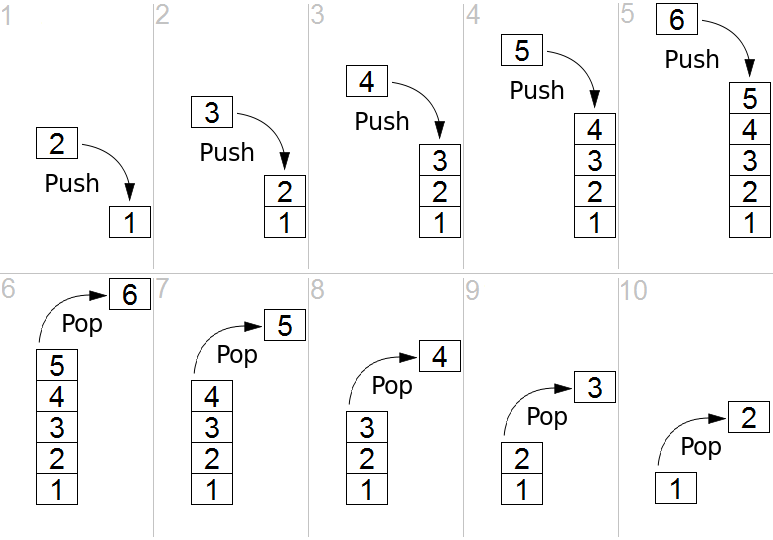
\includegraphics[width=0.8\textwidth]{Figures/Lifo_stack.png}
	\caption{\texttt{push()} and \texttt{pop()} over a stack.}
\end{figure}
\vfill
\end{frame}
%
\subsection{Simulating a Stack}
\begin{frame}
\vfill
You can simulate the behaviour of a stack with lists.
\vfill
\begin{table}[]
\begin{flushleft}
\begin{tabular}{ll}
\texttt{S = [ ]} &  \# start with an empty stack $\mathcal{S}_\emptyset$\\
\texttt{S.insert(0, 1)} &  \\
\texttt{S.insert(0, 2)} &  \# step 1 in previous slide\\
\texttt{S.insert(0, 3)} &  \# step 2 in previous slide\\
\texttt{S.insert(0, 4)} &  \# step 3 in previous slide\\
\texttt{S.insert(0, 5)} &  \# step 4 in previous slide\\
\texttt{S.insert(0, 6)} &  \# step 5 in previous slide\\
\texttt{S.pop(0)} &  \# step 6 in previous slide\\
\texttt{S.pop(0)} &  \# step 7 in previous slide\\
\texttt{S.pop(0)} &  \# step 8 in previous slide\\
\texttt{S.pop(0)} &  \# step 9 in previous slide\\
\texttt{S.pop(0)} &  \# step 10 in previous slide\\
\end{tabular}
\end{flushleft}
\end{table}
\vfill
\begin{block}{Recall}
\texttt{lst.insert(x, y)} inserts value \texttt{y} at position \texttt{x} in list \texttt{lst}.
\end{block}
\vfill
\end{frame}
%
\begin{frame}
\vfill
\begin{block}{Note}
Previously, we supposed that the head of the list is the top of the stack.\\
You can also assume that the tail of the list is the head of the stack.
\end{block}
\vfill
\begin{table}[]
\begin{flushleft}
\begin{tabular}{ll}
\texttt{S = [ ]} &  \# start with an empty stack $\mathcal{S}_\emptyset$\\
\texttt{S.append(1)} &  \\
\texttt{S.append(2)} &  \# step 1 in slide 4\\
\texttt{S.append(3)} &  \# step 2 in slide 4\\
\texttt{S.append(4)} &  \# step 3 in slide 4\\
\texttt{S.append(5)} &  \# step 4 in slide 4\\
\texttt{S.append(6)} &  \# step 5 in slide 4\\
\texttt{S.pop()} &  \# step 6 in slide 4\\
\texttt{S.pop()} &  \# step 7 in slide 4\\
\texttt{S.pop()} &  \# step 8 in slide 4\\
\texttt{S.pop()} &  \# step 9 in slide 4\\
\texttt{S.pop()} &  \# step 10 in slide 4\\
\end{tabular}
\end{flushleft}
\end{table}
\vfill
\end{frame}
% -----------------------------------------------------------------------------
\section{Queues}
\begin{frame}{Queues}
\vfill
The \textcolor{red}{queue} is another popular abstract data type in computer science.
\vfill
A queue is a sequence (collection) of elements where only the "oldest" element can be accessed.
\vfill
The allowed operations on a queue $\mathcal{Q}$ are the following:
\begin{itemize}
	\item \texttt{enqueue(}$e$\texttt{, }$\mathcal{Q}$\texttt{)}: adds a new element $e \in \mathcal{V}$, for any domain $\mathcal{V}$, at the beginning (back) of the queue $\mathcal{Q}$
	\item \texttt{dequeue(}$\mathcal{Q}$\texttt{)}: returns and removes the current element at the end (front) of the queue $\mathcal{Q}$.
\end{itemize}
Optionally, it is possible to define an additional operation:
\begin{itemize}
	\item \texttt{peek(}$\mathcal{Q}$\texttt{)}: reads the last element without modifying the queue.
\end{itemize}
\vfill
\end{frame}
%
\begin{frame}
\vfill
A special domain value is $\mathcal{Q}_\emptyset$, namely the empty queue.
\vfill
As $\mathcal{Q}_\emptyset$ has no elements:
\begin{itemize}
	\item \texttt{dequeue()} is not allowed
	\item \texttt{peek()} is not allowed.
\end{itemize}
\vfill
The queue is a FIFO (First-In, First-Out) data structure, because:
\begin{itemize}
	\item the first element that entered the queue (i.e., via \texttt{enqueue()})
	\item ... is the one that will be removed first (i.e., via \texttt{dequeue()})
\end{itemize}
\vfill
\end{frame}
%
\begin{frame}
\vfill
\begin{figure}
	\centering
	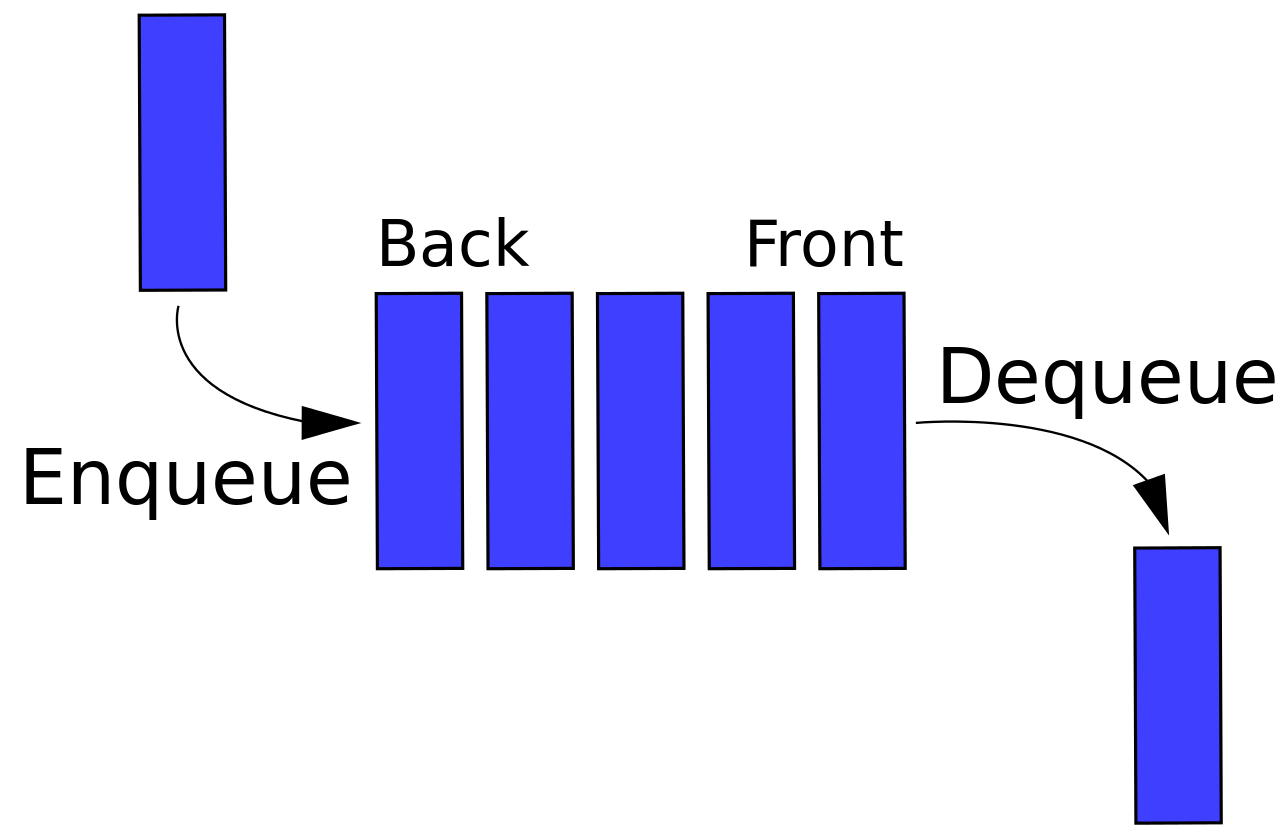
\includegraphics[width=0.8\textwidth]{Figures/Data_Queue.svg.png}
	\caption{Queues}
\end{figure}
\vfill
\end{frame}
%
\subsection{Simulating a Queue}
\begin{frame}
\vfill
You can simulate the behaviour of a queue with lists.
\vfill
\begin{table}[]
\begin{flushleft}
\begin{tabular}{ll}
\texttt{Q = [ ]} &  \# start with an empty queue $\mathcal{Q}_\emptyset$\\
\texttt{Q.insert(0, 1)} &  \# \texttt{insert} at the beginning = \texttt{enqueue}\\
\texttt{Q.insert(0, 2)} &  \\
\texttt{Q.insert(0, 3)} &  \\
\texttt{Q.insert(0, 4)} &  \\
\texttt{Q.insert(0, 5)} &  \\
\texttt{Q.insert(0, 6)} &  \\
\texttt{Q.pop()} &  \# \texttt{pop} at the end = \texttt{dequeue}\\
\texttt{Q.pop()} &  \\
\texttt{Q.pop()} &  \\
\texttt{Q.pop()} &  \\
\texttt{Q.pop()} &  \\
\end{tabular}
\end{flushleft}
\end{table}
\vfill
\begin{block}{Note}
Here we suppose that the head of the list is the beginning (back) of the queue and that the tail of the list is the end (front) of the queue.
\end{block}
\vfill
\end{frame}
%
\subsection{Queue vs. Stack}
\begin{frame}
\vfill
\begin{figure}
     \centering
     \begin{subfigure}{0.5\textwidth}
         \centering
         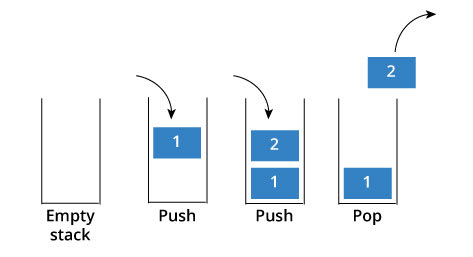
\includegraphics[width=\textwidth]{Figures/l8r4ic2gedi0j9obd7ix.jpg}
         \caption{Stack}
     \end{subfigure}

	\vspace{0.3cm}
     \begin{subfigure}{0.5\textwidth}
         \centering
         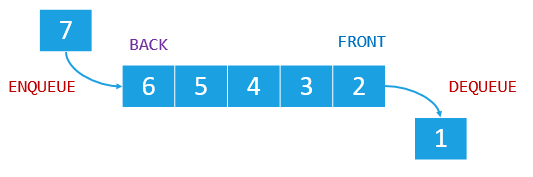
\includegraphics[width=\textwidth]{Figures/fcxri84smzo9m1pxbxj9.png}
         \caption{Queue}
     \end{subfigure}
        \caption{Queue vs. Stack (serious version)}
\end{figure}
\vfill
\end{frame}
%
\begin{frame}
\vfill
\begin{figure}
     \centering
     \begin{subfigure}[b]{0.3\textwidth}
         \centering
         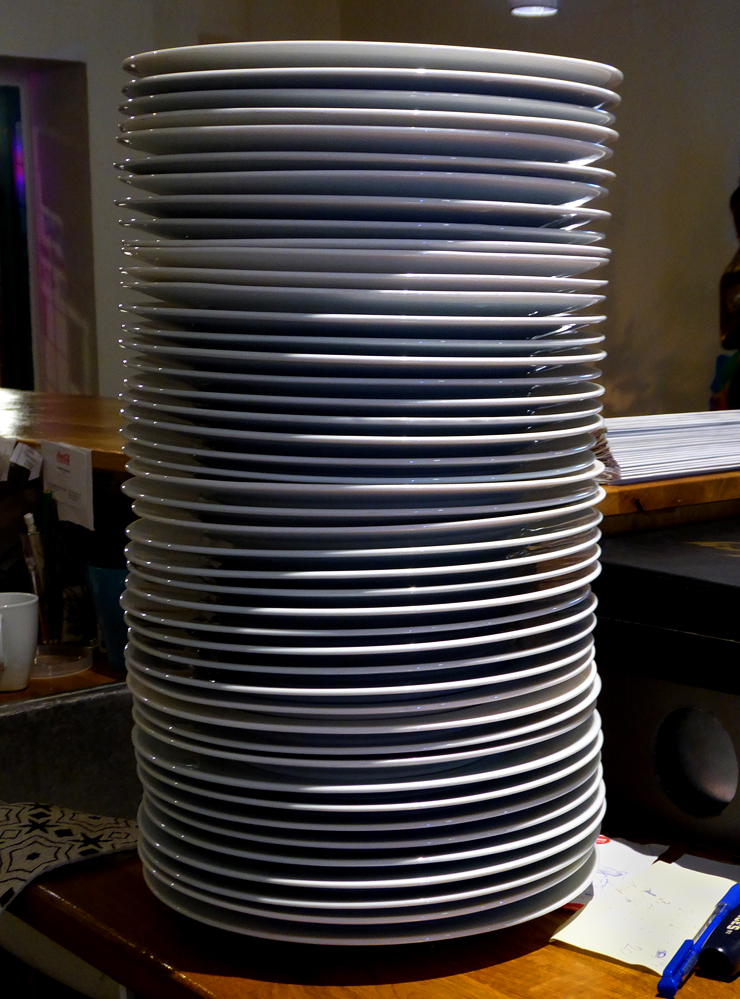
\includegraphics[width=\textwidth]{Figures/Tallrik_-_Ystad-2018.jpg}
         \caption{Stack}
     \end{subfigure}
     \hfill
     \begin{subfigure}[b]{0.6\textwidth}
         \centering
         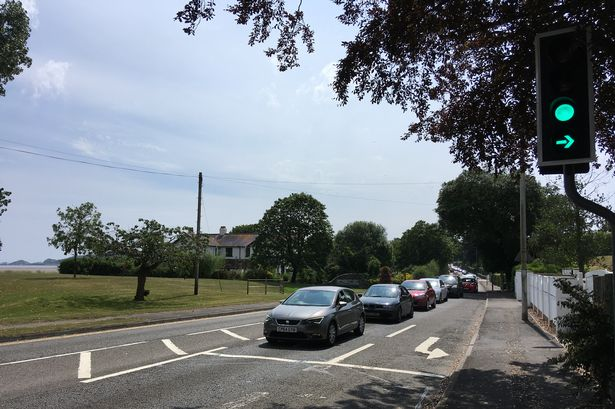
\includegraphics[width=\textwidth]{Figures/0_25203CE7-A5F0-48DF-8882-165CB0F63B2Fjpeg.jpg}
         \caption{Queue}
     \end{subfigure}
        \caption{Queue vs. Stack (not-so-serious version)}
\end{figure}
\vfill
\end{frame}
% -----------------------------------------------------------------------------
\section{Recursion}
\begin{frame}{Recursion}
\vspace{-0.2cm}
\vfill
\begin{center}
\begin{figure}
	\centering
	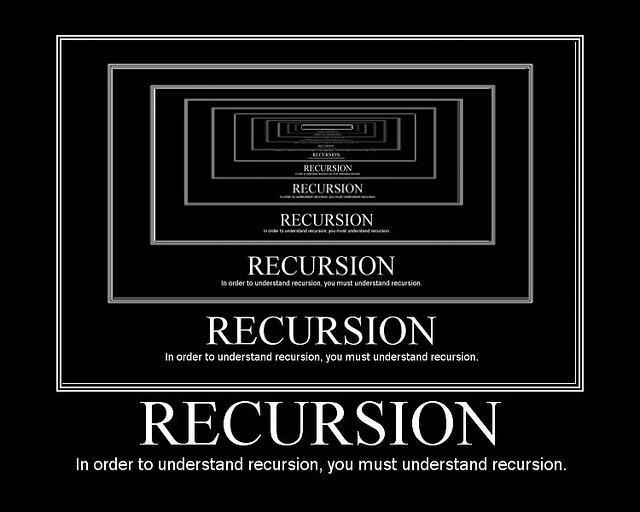
\includegraphics[width=0.8\textwidth]{Figures/recursionimage.jpg}
\end{figure}
\end{center}
\vfill
\end{frame}
%
\subsection{Recursion and Problem Solving}
\begin{frame}
\vfill
When designing the solution of a problem
\begin{center}
	\textcolor{red}{... try to solve the problem assuming that you have \textit{already solved it}!}
\end{center}
\vfill
How is that possible?
\begin{center}
	\textcolor{red}{Define the solution of a problem instance in terms of the solution of \textit{smaller} problem instances.}
\end{center}
\vfill
Practically speaking:
\begin{center}
	\textcolor{red}{The function that computes the solution will \textit{invoke itself} (once or more than once) from inside its body.}
\end{center}
\vfill
\end{frame}
%
\subsection{Examples}
\begin{frame}
\vfill
\begin{figure}
     \centering
     \begin{subfigure}[b]{0.3\textwidth}
         \centering
         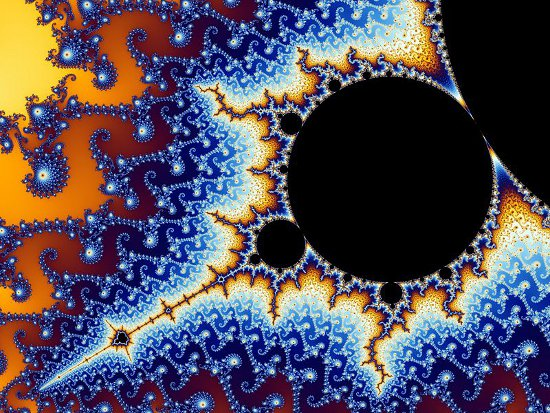
\includegraphics[width=\textwidth]{Figures/800px-Mandel_zoom_08_satellite_antenna.jpg}
         \caption{Mandelbrot Set}
     \end{subfigure}
     \qquad
     \begin{subfigure}[b]{0.3\textwidth}
         \centering
         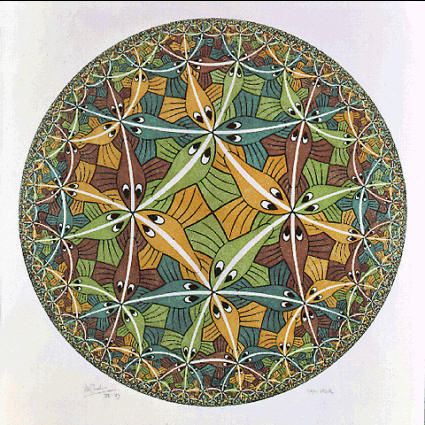
\includegraphics[width=0.9\textwidth]{Figures/escher-fish.jpg}
         \caption{Escher's \textit{Circle Limit III}}
	\end{subfigure}

     \begin{subfigure}[b]{0.3\textwidth}
         \centering
         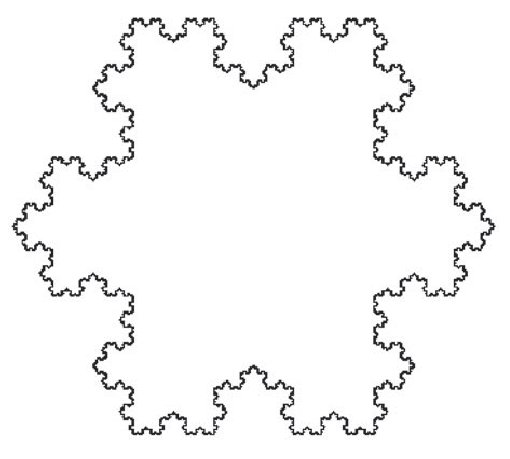
\includegraphics[width=\textwidth]{Figures/An-image-of-the-Koch-snowflake-a-fractal-with-fractal-dimension-d-126-From_W640.jpg}
         \caption{Koch Snowflake}
     \end{subfigure}
     \qquad
     \begin{subfigure}[b]{0.3\textwidth}
         \centering
         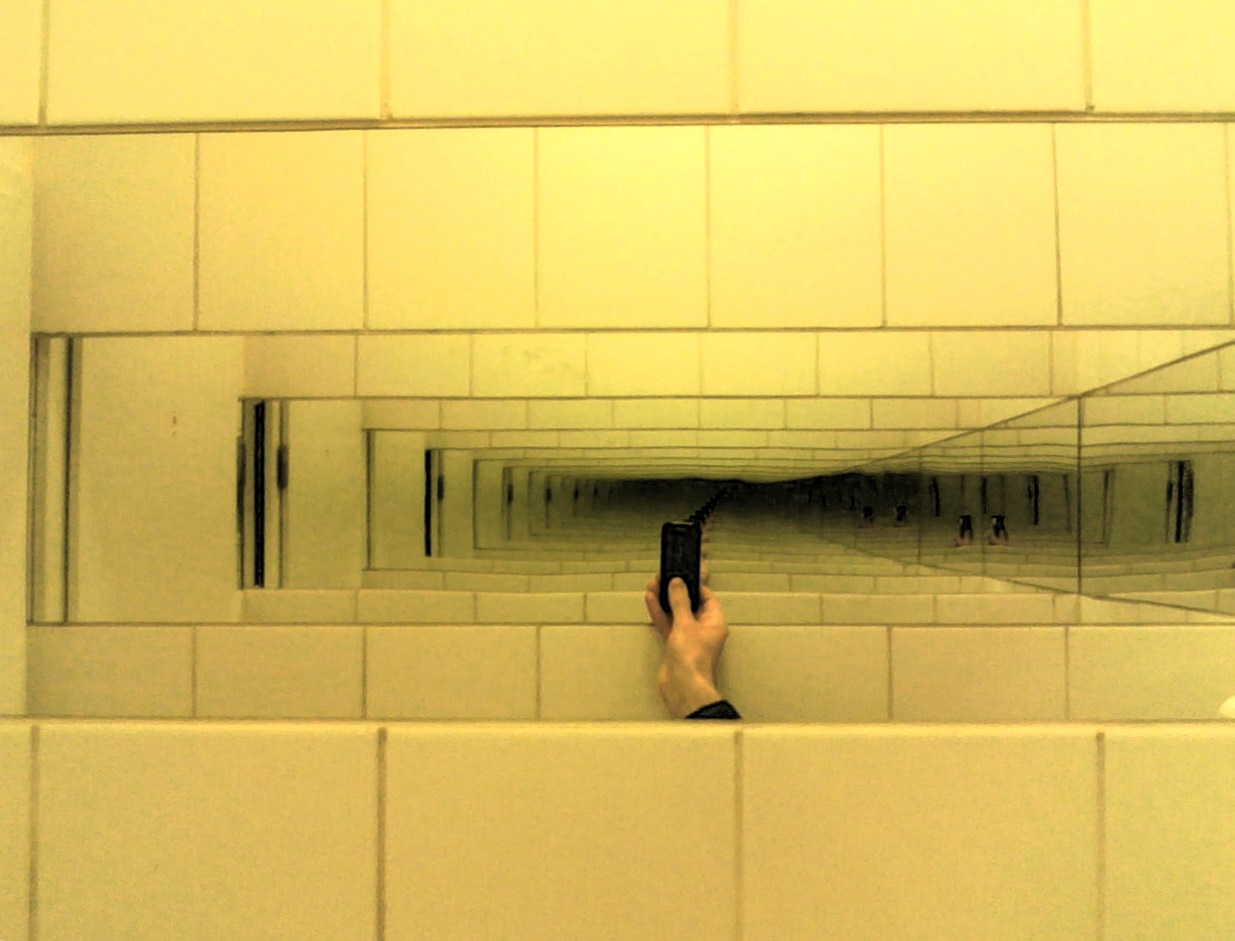
\includegraphics[width=\textwidth]{Figures/Infinity_Mirror_Effect.jpg}
         \caption{Parallel Mirrors}
     \end{subfigure}
        \caption{Real-world recursion}
\end{figure}
\vfill
\end{frame}
%
\begin{frame}
\vfill
A more practical example? Computing the factorial of a number $n$.
\begin{equation*}
	n! = n \cdot (n-1) \cdot (n-2) \cdot \ldots \cdot 1
\end{equation*}
%or, similarly,
%\begin{equation*}
%	n! = 1 \cdot 2 \cdot 3 \cdot \ldots \cdot (n-1) \cdot n
%\end{equation*}
Back-of-the-envelope calculation: $5!$
\begin{equation*}
	5! = \underbrace{5 \cdot \underbrace{4 \cdot \underbrace{3 \cdot \underbrace{2 \cdot \underbrace{1}_\text{$1!$}}_\text{$2 \cdot 1!$}}_\text{$3 \cdot 2!$}}_\text{$4 \cdot 3!$}}_\text{$5 \cdot 4!$}
\end{equation*}
We can spot the following pattern:
\begin{equation*}
	n! = n \cdot (n-1)!
\end{equation*}
with base case
\begin{equation*}
	0! = 1
\end{equation*}
\vfill
\end{frame}
%
\subsection{Recursion and Problem Solving (pt.2)}
\begin{frame}
\vfill
In order to use a recursive approach:
\begin{enumerate}
	\item you must be able to \textcolor{red}{decompose} the problem into problems of the same type
	\item you must find a \textcolor{red}{relation} that connects a given problem to the solution of similar subproblems
	\item you need to know the solution of a special case of the problem (the \textcolor{red}{base case}, where the recursion terminates).
\end{enumerate}
\vfill
Take the factorial example:
\begin{enumerate}
	\item multiplication between two numbers
	\item multiplication between $n$ and the already-known $(n-1)!$
	\item the base case is $0!=1$
\end{enumerate}
\vfill
\end{frame}
%
\subsection{Issues with Recursion}
\begin{frame}
\vfill
There are two major issues with recursion:
\begin{enumerate}
	\item \textcolor{red}{Infinite recursion}
	\begin{itemize}
		\item missing base case?
		\item function called with wrong arguments?
	\end{itemize}
	For example, what happens if we do \texttt{(-1)!} ?\\
	... more on this later
	\item \textcolor{red}{Un-responsiveness}
	\begin{itemize}
		\item your code can easily become very slow, also with "easy" input parameters
		\item ... more on memory management later
	\end{itemize}
\end{enumerate}
\vfill
\begin{block}{Note}
Python is quite good at catching infinite recursions: it has a dedicated error.\\
\texttt{\textcolor{red}{RecursionError}: maximum recursion depth exceeded in comparison}
\end{block}
\vfill
\end{frame}
% -----------------------------------------------------------------------------
\section{Memory Management}
\subsection{Case Study: \texttt{countdown}}
\begin{frame}{Memory Management}
\vfill
Write a recursive function \texttt{countdown(n)} that takes a positive integer \texttt{n} and prints the countdown. As the countdown reaches 0, prints \texttt{Blastoff!} and quits.
\begin{table}[]
\begin{flushleft}
\begin{tabular}{ll}
\texttt{>{}>{}> def countdown(n):} &  \\
\texttt{>{}>{}> \qquad if n==0:} &  \\
\texttt{>{}>{}> \qquad\qquad print("Blastoff!")} &  \\
\texttt{>{}>{}> \qquad else:} &  \\
\texttt{>{}>{}> \qquad\qquad print(n)} &  \\
\texttt{>{}>{}> \qquad\qquad countdown(n-1)} &  \\
\texttt{ } &  \\
\texttt{>{}>{}> countdown(3)} &  \\
\texttt{3} &  \\
\texttt{2} &  \\
\texttt{1} &  \\
\texttt{Blastoff!} &  \\
\end{tabular}
\end{flushleft}
\end{table}
\vfill
\end{frame}
%
\begin{frame}
\vfill
% What's going on here?
% \begin{enumerate}
% 	\item The execution of \texttt{countdown} begins with \texttt{n=3}, and since \texttt{n} is greater than \texttt{0}, it outputs the value \texttt{3}, and then calls itself ...
% 	\begin{enumerate}[2]
% 	\item The execution of \texttt{countdown} begins with \texttt{n=2}, and since \texttt{n} is greater than \texttt{0}, it outputs the value \texttt{2}, and then calls itself ...
% 		\begin{enumerate}[3]
% 		\item The execution of \texttt{countdown} begins with \texttt{n=1}, and since \texttt{n} is greater than \texttt{0}, it outputs the value \texttt{1}, and then calls itself ...
% 			\begin{enumerate}[4]
% 			\item The execution of \texttt{countdown} begins with \texttt{n=0}, and since \texttt{n} is not greater than \texttt{0}, it outputs \texttt{Blastoff!} and then returns.
% 			\end{enumerate}
% 		\end{enumerate}
% 		\begin{enumerate}[5]
% 		\item The countdown that got \texttt{n=1} returns.
% 		\end{enumerate}
% 		\end{enumerate}
% 		\begin{enumerate}[6]
% 		\item The countdown that got \texttt{n=2} returns.
% 		\end{enumerate}
% 	\end{enumerate}
% 	\begin{enumerate}[7]
% 		\item The countdown that got \texttt{n=3} returns.
% 	\end{enumerate}
What's going on here?
\begin{enumerate}
	\item The execution of \texttt{countdown} begins with \texttt{n=3}, and since \texttt{n} is greater than \texttt{0}, it outputs the value \texttt{3}, and then calls itself ...
	\setlength{\itemindent}{0.1in}
	\item The execution of \texttt{countdown} begins with \texttt{n=2}, and since \texttt{n} is greater than \texttt{0}, it outputs the value \texttt{2}, and then calls itself ...
	\setlength{\itemindent}{0.2in}
	\item The execution of \texttt{countdown} begins with \texttt{n=1}, and since \texttt{n} is greater than \texttt{0}, it outputs the value \texttt{1}, and then calls itself ...
	\setlength{\itemindent}{0.3in}
	\item The execution of \texttt{countdown} begins with \texttt{n=0}, and since \texttt{n} is not greater than \texttt{0}, it outputs \texttt{Blastoff!} and then returns.
	\setlength{\itemindent}{0.2in}
	\item The countdown that got \texttt{n=1} returns.
	\setlength{\itemindent}{0.1in}
	\item The countdown that got \texttt{n=2} returns.
	\setlength{\itemindent}{0.0in}
	\item The countdown that got \texttt{n=3} returns.
\end{enumerate}
And we are back into the \texttt{main} script.
\vfill
\end{frame}
%
\begin{frame}
\vfill
\begin{block}{Recall}
Every time a function gets called, Python creates a new function frame, which contains the function's local variables and parameters.
\end{block}
For a recursive function, there might be more than one frame at the same time. Python organises those frames as a \textcolor{red}{stack}.
\vfill
\begin{figure}
	\centering
	
\includegraphics[width=0.25\textwidth]{Figures/book007.png}
	\caption{Stack diagram for \texttt{countdown(3)}.}
	\label{stack}
\end{figure}
\vfill
\end{frame}
%
\begin{frame}
\vfill
How does the stack in Figure \ref{stack} works?
\begin{enumerate}
	\item (as usual) at the top of the stack is the frame for the \texttt{main}\footnote{In our case, it is empty because we did not create any variables in \texttt{main} or pass any arguments to it.}
	\item we call \texttt{countdown(3)}, so there is a new frame in the stack
	\item \texttt{countdown(3)} calls \texttt{countdown(2)}, so there is a new frame in the stack
	\item \texttt{countdown(2)} calls \texttt{countdown(1)}, so there is a new frame in the stack
	\item \texttt{countdown(1)} calls \texttt{countdown(0)}, so there is a new frame in the stack
	\item \texttt{countdown(0)} does not make any further calls, so no more frames
\end{enumerate}
We did a bunch of \texttt{push}es, now we must do some \texttt{pop}s:
\begin{enumerate}
	\item \texttt{countdown(0)} finishes its execution (i.e., prints \texttt{Blastoff!} without doing anything else). Its frame is erased.
	\item the control goes back to \texttt{countdown(1)}, which finishes its execution. Its frame is erased.
	\item the control goes back to \texttt{countdown(2)}, which finishes its execution. Its frame is erased.
	\item the control goes back to \texttt{countdown(3)}, which finishes its execution. Its frame is erased.
	\item the control goes back to the \texttt{main}.
\end{enumerate}
\vfill
\end{frame}
%------------------------------------------------------------------------------
\section{Exercises}
\subsection{\texttt{factorial}}
\begin{frame}{Exercises}
\vfill
Write a recursive function \texttt{factorial(n)} that takes as input a positive integer \texttt{n} and returns $n!$.
\vfill
\begin{table}[]
\begin{flushleft}
\begin{tabular}{ll}
\texttt{>{}>{}> def factorial(n):} &  \\
\texttt{>{}>{}> \qquad if n==0:} &  \\
\texttt{>{}>{}> \qquad\qquad return 1} &  \\
\texttt{>{}>{}> \qquad else:} &  \\
\texttt{>{}>{}> \qquad\qquad return n * factorial(n-1)} &  \\
\texttt{ } &  \\
\texttt{>{}>{}> output = factorial(5)} &  \\
\texttt{>{}>{}> print(output)} &  \\
\texttt{120} &  \\
\end{tabular}
\end{flushleft}
\end{table}
\vfill
\begin{block}{Warning}
What happens when calling \texttt{factorial(-1)}?
\end{block}
\vfill
\end{frame}
%
\begin{frame}
\vfill
\begin{figure}
	\centering
	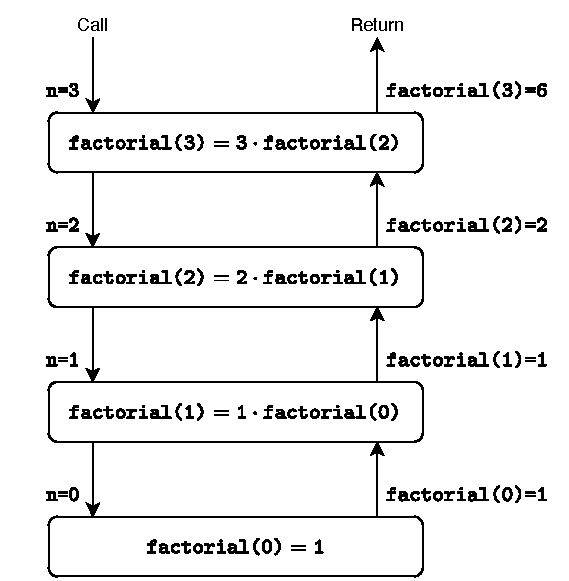
\includegraphics[width=0.6\textwidth]{Figures/stackframes_factorial}
	\caption{Stack diagram for \texttt{factorial(3)}.}
\end{figure}
\vfill
\end{frame}
%
\subsection{\texttt{palindrome}}
\begin{frame}
\vfill
Write a recursive function \texttt{palindrome(s)} that takes as input a string \texttt{s} and returns \texttt{True} if \texttt{s} is palindrome\footnote{A word (or any other sequence of characters) is said to be \textit{palindrome} if it reads the same backward as forward.} and \texttt{False} otherwise.
\vfill
Decomposition strategy: let \texttt{s} be \texttt{"racecar"}
\begin{table}[]
\begin{tabular}{ll}
\texttt{\textcolor{red}{r}aceca\textcolor{red}{r}} &  same letter \cmark \\
\texttt{\textcolor{blue}{a}cec\textcolor{blue}{a}} &  same letter \cmark \\
\texttt{\textcolor{magenta}{c}e\textcolor{magenta}{c}} &  same letter \cmark \\
\texttt{e} &  trivial \cmark \\
\end{tabular}
\end{table}
and now let \texttt{s} be \texttt{"rediviuer"}
\begin{table}[]
\begin{tabular}{ll}
\texttt{\textcolor{red}{r}ediviue\textcolor{red}{r}} &  same letter \cmark \\
\texttt{\textcolor{blue}{e}diviu\textcolor{blue}{e}} &  same letter \cmark \\
\texttt{\textcolor{magenta}{d}ivi\textcolor{magenta}{u}} &  different letter \xmark \\
%\texttt{\textcolor{green}{i}v\textcolor{green}{i}} &  same letter \cmark \\
%\texttt{v} &  trivial \cmark \\
\end{tabular}
\end{table}
Hence, \texttt{"racecar"} is palindrome, but \texttt{"rediviuer"} it's not.
\vfill
\end{frame}
%
\begin{frame}
\vfill
\begin{table}[]
\begin{flushleft}
\begin{tabular}{ll}
\texttt{>{}>{}> def palindrome(s):} &  \\
\texttt{>{}>{}> \qquad if len(s) <= 1:} &  \\
\texttt{>{}>{}> \qquad\qquad return True} &  \\
\texttt{>{}>{}> \qquad else:} &  \\
\texttt{>{}>{}> \qquad\qquad return (s[0] == s[-1]) and palindrome(s[1:-1])} &  \\
\texttt{ } &  \\
\texttt{>{}>{}> output1 = palindrome("racer")} &  \\
\texttt{>{}>{}> print(output1)} &  \\
\texttt{True} &  \\
\texttt{>{}>{}> output2 = palindrome("rediviuer")} &  \\
\texttt{>{}>{}> print(output2)} &  \\
\texttt{False} &  \\
\end{tabular}
\end{flushleft}
\end{table}
\vfill
\end{frame}
%
\begin{frame}
\vfill
\begin{figure}
	\centering
	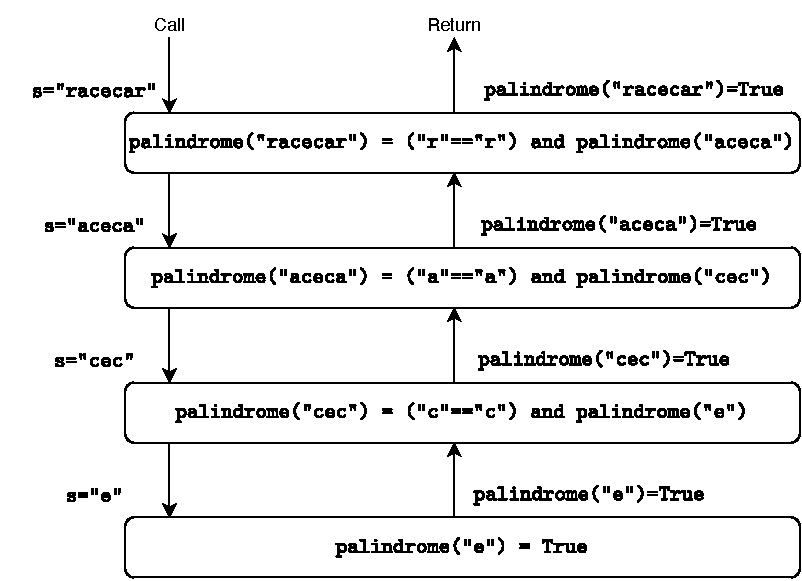
\includegraphics[width=0.8\textwidth]{Figures/stackframes_palindrome}
	\caption{Stack diagram for \texttt{palindrome("racecar")}.}
\end{figure}
\vfill
\end{frame}
%
\begin{frame}
\vfill
\begin{figure}
	\centering
	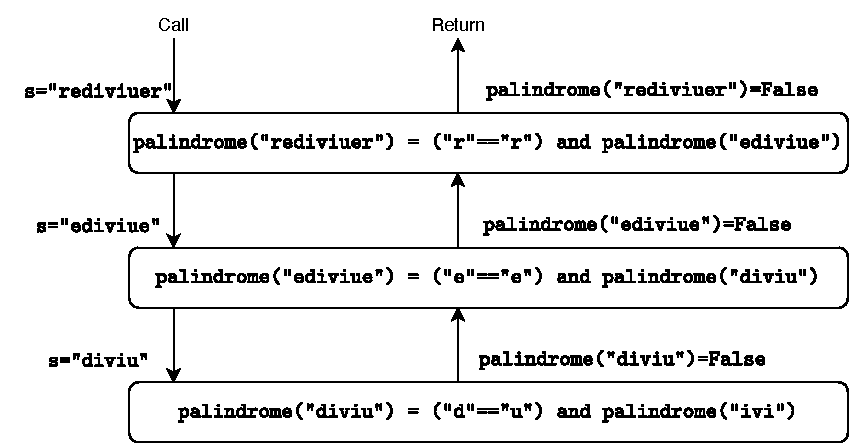
\includegraphics[width=0.85\textwidth]{Figures/stackframes_palindrome2}
	\caption{Stack diagram for \texttt{palindrome("rediviuer")}.}
\end{figure}
\vfill
\end{frame}
%
\subsection{\texttt{fibonacci}}
\begin{frame}
\vfill
Write a recursive function \texttt{fibonacci(n)} that takes as input a positive integer \texttt{n} and returns the $n$\textsuperscript{th} Fibonacci number.
\vfill
%\begin{table}[]
%\begin{flushleft}
%\begin{tabular}{ll}
%\texttt{>{}>{}> def fibonacci(n):} &  \\
%\texttt{>{}>{}> \qquad if n==0:} &  \\
%\texttt{>{}>{}> \qquad\qquad return 1} &  \\
%\texttt{>{}>{}> \qquad else:} &  \\
%\texttt{>{}>{}> \qquad\qquad return n * factorial(n-1)} &  \\
%\texttt{ } &  \\
%\texttt{>{}>{}> output = factorial(5)} &  \\
%\texttt{>{}>{}> print(output)} &  \\
%\texttt{120} &  \\
%\end{tabular}
%\end{flushleft}
%\end{table}
%\vfill
\begin{block}{Recall}
Each number in the Fibonacci sequence is given by the sum of the two preceding ones:\\
\texttt{0} \texttt{1} \textcolor{blue}{\texttt{1} \texttt{2} \texttt{3} \texttt{5} \texttt{8} \texttt{11} ...}
\end{block}
\vfill
Decomposition strategy: \texttt{fibonacci(n)} with \texttt{n=5}\footnote{By coincidence, the 5\textsuperscript{th} Fibonacci number is 5.}.
%\begin{equation*}
%	\underbrace{\texttt{fibonacci(5)}}_{\underbrace{\texttt{fibonacci(4)}}_{\texttt{fibonacci(3)}+\texttt{fibonacci(2)}} + \underbrace{\texttt{fibonacci(3)}}_{\texttt{fibonacci(2)}+\texttt{fibonacci(1)}}}
%\end{equation*}
\begin{equation*}
	\underbrace{5}_{\textstyle \underbrace{3}_{\textstyle\underbrace{2}_{\textstyle 1+1}+1} + \underbrace{2}_{\textstyle 1+1}}
\end{equation*}
\vfill
\end{frame}
%
\begin{frame}
\vfill
\begin{table}[]
\begin{flushleft}
\begin{tabular}{ll}
\texttt{>{}>{}> def fibonacci(n):} &  \\
\texttt{>{}>{}> \qquad if n in [0, 1]:} &  \\
\texttt{>{}>{}> \qquad\qquad return n} &  \\
\texttt{>{}>{}> \qquad else:} &  \\
\texttt{>{}>{}> \qquad\qquad return (fibonacci(n-1) + fibonacci(n-2))} &  \\
\texttt{ } &  \\
\texttt{>{}>{}> output = fibonacci(5)} &  \\
\texttt{>{}>{}> print(output)} &  \\
\texttt{5} &  \\
\end{tabular}
\end{flushleft}
\end{table}
\vfill
\end{frame}
%
\begin{frame}
\vfill
\begin{figure}
	\centering
	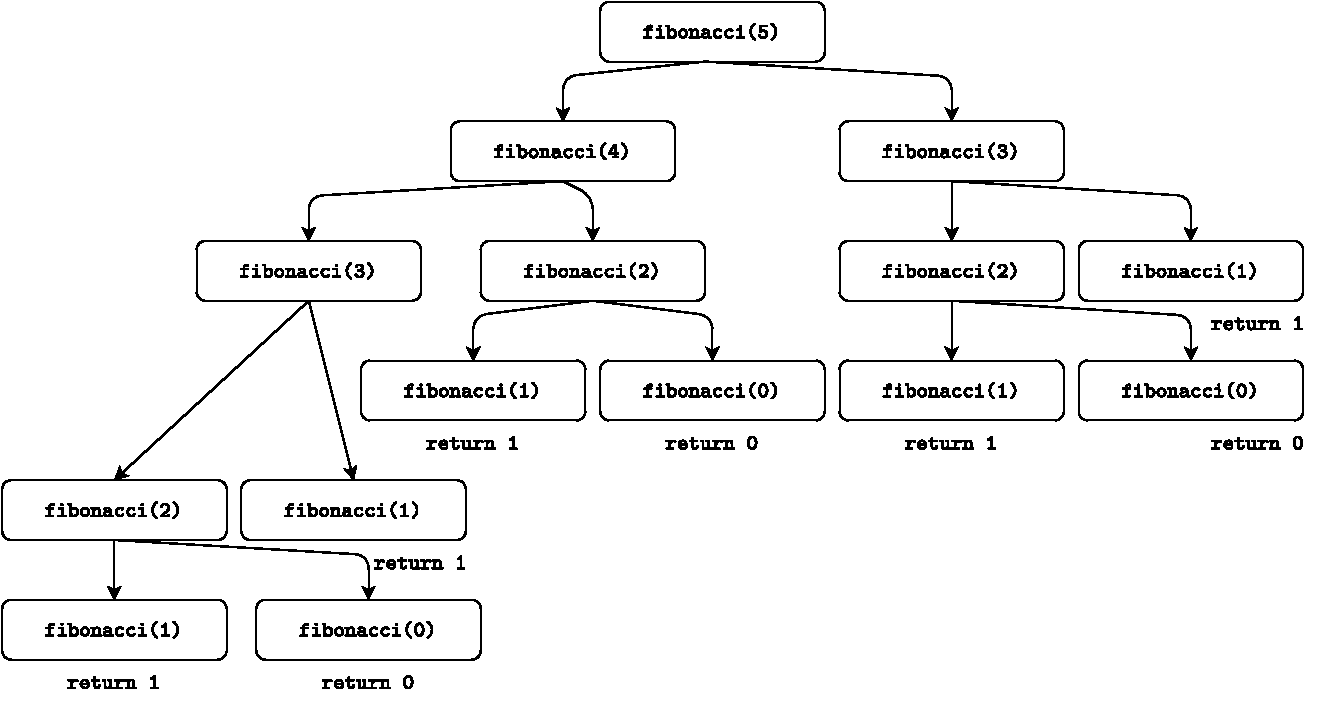
\includegraphics[width=\textwidth]{Figures/stackframes_fibonacci}
	\caption{Call Stack diagram for \texttt{fibonacci(5)}.}
\end{figure}
\vfill
\end{frame}
%
\begin{frame}
\vfill
\begin{figure}
	\centering
	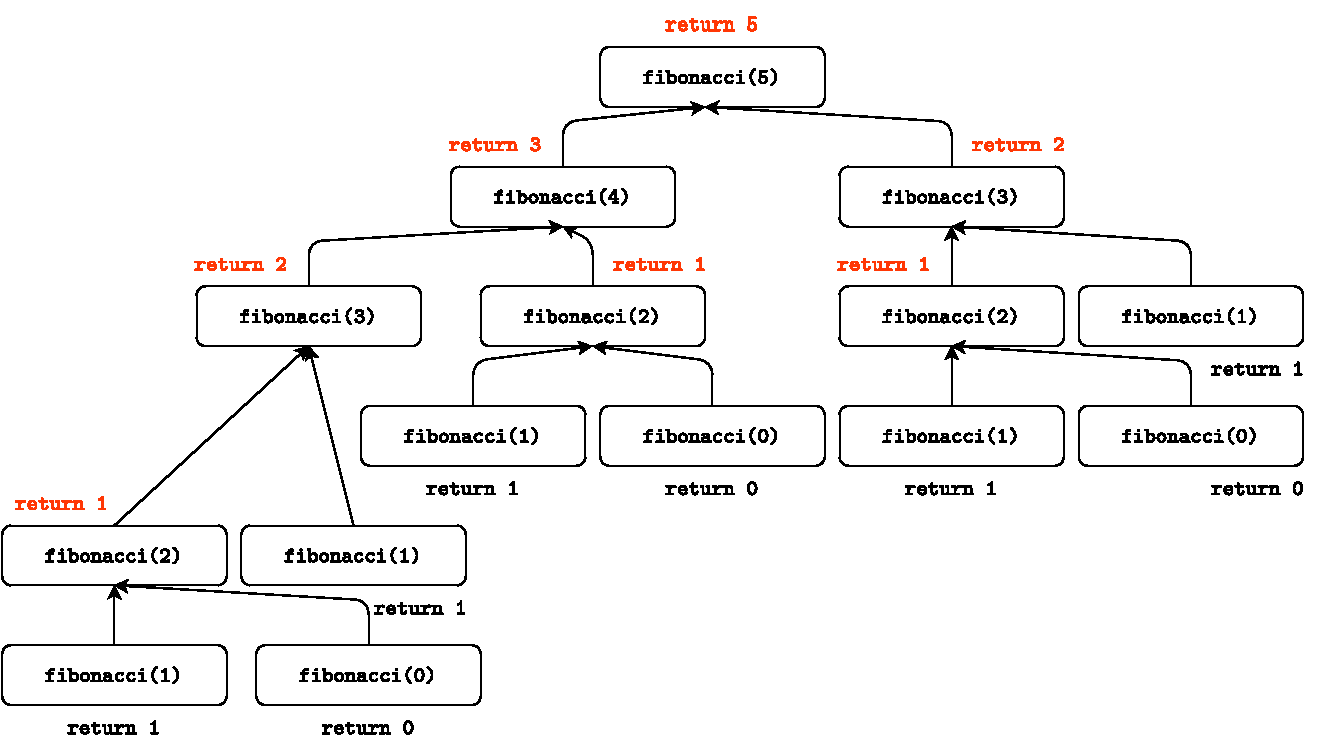
\includegraphics[width=\textwidth]{Figures/stackframes_fibonacci2}
	\caption{Return Stack diagram for \texttt{fibonacci(5)}.}
\end{figure}
\vfill
\end{frame}
%------------------------------------------------------------------------------
%\section{References}
%\begin{frame}[allowframebreaks]{References}
%%\bibliographystyle{apacite}
%\printbibliography[heading=none]
%\end{frame}
\section{References}
\begin{frame}{References}
\begin{itemize}
	\item Guttag, J. V. (2013). \textit{Introduction to Computation and Programming using Python (Revised and Expanded Edition)}. MIT Press. [Section 4.3]
	\item Downey, A. (2015). \textit{Think Python}. Green Tea Press ed. 2nd. [Sections 5.8--5.10]
\end{itemize}
\end{frame}
%------------------------------------------------------------------------------
\section{Acknowledgments}
\begin{frame}{Acknowledgments}
\begin{itemize}
	% \item Prof. Irene Finocchi (LUISS University)\\
	% \quad \textit{Introduction to Computer Programming} Lecture Notes (2020-2021)
	\item \url{https://en.wikipedia.org/wiki/Stack_(abstract_data_type)}
	\item \url{https://en.wikipedia.org/wiki/Queue_(abstract_data_type)}
	\item \url{https://www.walesonline.co.uk/news/wales-news/swansea-roads-cars-traffic-bikes-21148566}
\end{itemize}
\end{frame}
%------------------------------------------------------------------------------
%\subsection{Sites legais}
%\begin{frame}{Sites legais}
%  Want to know more? See!
%  \begin{itemize}
%    \item Browse in my page \url{http://www.ezefranca.com}.
%    \item Browse on BCC page \url{http://www.sp.senac.br/bcc}.
%    \item Thanks WriteLaTeX from Support! \url{http://www.writelatex.com}.
%  \end{itemize}
%
%\end{frame}
%------------------------------------------------------------------------------

% -----------------------------------------------------------------------------
\end{document}
%-----------------------------------------------Este comentario nunca aparecera
